\section{Experiments}
\label{sec:exp}

\subsection{Setup}
\label{sec:setup}

\paragraph{Models.} The main experiments use the Olmo~3 RL-Zero family
\citep{olmo2025olmo3}. The base is Olmo-3-1025-7B, and the teachers are the
final checkpoints of Olmo-3.1-7B-RL-Zero-Math and Olmo-3.1-7B-RL-Zero-Code,
each obtained by reinforcement learning from that base on a single domain.

\paragraph{Rollouts and statistics.} For mathematics the teacher answers 256
training problems from DAPO-Math-17k \citep{yu2025dapo}; for code, 256
training problems from the DeepCoder training set \citep{luo2025deepcoder},
with the instruction used by EvalPlus. Each problem is answered once.
Mathematics is sampled at temperature 0.7 and top-$p$ 0.9 with a limit of
31{,}744 new tokens, code at temperature 1.0 and top-$p$ 1.0 with a limit of
32{,}768, matching evaluation. No evaluation problem is used. Selection keeps
the 175 mathematics answers that are correct, finished and loop-free, and the
92 code answers that pass every test of their problem. We use $\alpha=0.9$
and equal domain weights.

\paragraph{Evaluation.} Mathematics: AIME24, AIME25 and HMMT25, the latter
two from MathArena \citep{balunovic2025matharena}, with accuracy averaged
over four sampled answers per problem and graded by rule, rejected answers
being re-checked by a model verifier (CompassVerifier-3B); and the two larger
benchmarks, MATH-500 \citep{hendrycks2021math} and OlympiadBench
\citep{he2024olympiadbench}, with one sampled answer per problem. Code:
HumanEval+ and MBPP+ under EvalPlus
\citep{chen2021codex,austin2021mbpp,liu2023evalplus}, with one sampled answer
per problem. Released checkpoints are evaluated in bfloat16, the format they
are released in, and fused models in float16 (Section~\ref{sec:precision});
Appendix~\ref{app:eval} gives the full protocol.

\paragraph{Baselines.} The base model and each teacher. Task arithmetic with
unit coefficients, $\Wb+\dd_{\text{math}}+\dd_{\text{code}}$
\citep{ilharco2023task}, is the weight-only reference;
Section~\ref{sec:ablations} adds a low-rank variant of it and closed-form
variants that differ in the rollouts they use.

\begin{table}[t]
\centering\small
\setlength{\tabcolsep}{4.8pt}
\begin{tabular}{@{}lcccccccc@{}}
\toprule
 & \multicolumn{5}{c}{Mathematics} & \multicolumn{2}{c}{Code} & \\
\cmidrule(lr){2-6}\cmidrule(lr){7-8}
Model & MATH-500 & OlympiadBench & AIME24 & AIME25 & HMMT25 & HumanEval+ & MBPP+ & Mean \\
\midrule
Base model & 63.4 & 33.4 & 15.8 & 10.0 & 8.3 & 45.7 & 44.2 & 31.6 \\
Math specialist & \textbf{91.8} & 68.7 & \textbf{50.0} & \textbf{43.3} & \textbf{30.8} & 71.3 & 62.4 & 59.8 \\
Code specialist & 85.6 & 62.5 & 26.7 & 30.0 & 15.0 & \textbf{86.0} & \textbf{69.3} & 53.6 \\
\rowcolor{oursrow}[\tabcolsep][\tabcolsep]\method (ours) & 90.8 & \textbf{69.4} & \textbf{50.0} & 38.3 & 27.5 & 84.1 & 67.5 & \textbf{61.1} \\
\bottomrule
\end{tabular}
\caption{\textbf{One generalist, ahead of both specialists on average (Olmo~3 7B).}
Accuracy (\%). AIME24, AIME25 and HMMT25 average four sampled answers per
problem; MATH-500, OlympiadBench, HumanEval+ and MBPP+ use one. Released
checkpoints are evaluated in bfloat16 and the fused model in float16. The mean
is taken over the seven benchmarks before rounding. The best value of each
column is in bold.}
\label{tab:main}
\end{table}

\subsection{Main results}
\label{sec:main}

Figure~\ref{fig:teaser} and Table~\ref{tab:main} give the main comparison.
The fused model has the highest mean accuracy of the four models
(Figure~\ref{fig:teaser}c): built without a gradient step, it is on average
better than either specialist it was built from. The reason is a trade-off
that each specialist carries and the fused model does not. Each specialist
is far ahead on its own domain and far behind on the other; \method is close
to the specialist of the domain on every benchmark
(Figure~\ref{fig:teaser}b), and in the plane of mathematics against code it
sits beside the corner set by the two specialists' own-domain scores
(Figure~\ref{fig:teaser}a). It equals the mathematics specialist on AIME24
and is slightly ahead of it on OlympiadBench, is nearly level with the
specialist of the domain on MATH-500 and on both code benchmarks, and keeps
most of what reinforcement learning added on every benchmark. It is the only
model that is never far from the best score, and its lead in mean accuracy
does not come from the benchmark count:
weighting the two domains equally widens it (Figure~\ref{fig:teaser}a).

None of this required training. The procedure is one generation pass and one
teacher-forced pass per specialist, followed by a linear solve per layer. It
keeps no optimizer state, has no learning rate to tune, and finishes in a few
GPU-hours per specialist (Table~\ref{tab:cost} in Appendix~\ref{app:eval}).
Training-based on-policy distillation spends the same kind of forward
computation at every update and adds a backward pass each time. For
specialists that share a base model, the closed form reaches a consolidated
model at roughly the cost of collecting such data once. Its advantage over
weight arithmetic is on hard problems: task arithmetic costs even less, but
falls short on AIME25, where the closed form with clean rollouts matches the
specialist in the same format (Section~\ref{sec:ablations}).

On AIME25 the fused model is within a point of the mathematics specialist
once both are scored in float16 (Table~\ref{tab:abl-aime});
Table~\ref{tab:main} scores the released checkpoints in their native format.
The three competition benchmarks have thirty problems each, so differences
of a few points are within what they resolve.

\subsection{Case study}
\label{sec:cases}

\begin{figure}[t]
\centering\footnotesize
\setlength{\fboxsep}{4pt}\setlength{\fboxrule}{0.7pt}
\fcolorbox{cink}{cice}{\parbox{\dimexpr\textwidth-2\fboxsep-2\fboxrule}{%
\textbf{Problem (HMMT25).} In a two-dimensional cave with a parallel floor
and ceiling, two stalactites of lengths 16 and 36 hang perpendicularly from
the ceiling, while two stalagmites of heights 25 and 49 grow perpendicularly
from the ground. If the tips of these four structures form the vertices of a
square in some order, compute the height of the cave. \hfill
\textbf{Answer: 63}}}

\vspace{4pt}
\begin{minipage}[t]{0.492\textwidth}
\fcolorbox{cnavy}{white}{\parbox[t]{\dimexpr\linewidth-2\fboxsep-2\fboxrule}{%
\textbf{\textcolor{cnavy}{\method: answers 63, correct}} \hfill 3 of 4 samples\\[3pt]
\emph{``Suppose that the four points form a square. Therefore, the midpoints
of the diagonals must coincide.''}\\[1pt]
\hspace*{1em}$\downarrow$\\[1pt]
\emph{``Midpoint of AB: (\,\dots, $H-26$). Midpoint of CD: (\,\dots, 37).''}\\[1pt]
\hspace*{1em}$\downarrow$\\[1pt]
\emph{``\dots\ their y-coordinates must satisfy $H-26=37\Rightarrow H=63$.
\dots\ Wait, this seems to work!''}\\[1pt]
\hspace*{1em}$\downarrow$\\[1pt]
\emph{``Thus, the height of the cave is 63.''}}}
\end{minipage}\hfill
\begin{minipage}[t]{0.492\textwidth}
\fcolorbox{crose}{white}{\parbox[t]{\dimexpr\linewidth-2\fboxsep-2\fboxrule}{%
\textbf{\textcolor{crose}{Math specialist: answers 61, wrong}} \hfill 0 of 4 samples\\[3pt]
\emph{``$(y-x)^2+400=(y-x)^2+576$, which implies $400=576$, which is
impossible. Hmm, so this approach is invalid.''}\\[1pt]
\hspace*{1em}$\downarrow$\\[1pt]
\emph{``I think I have to concede and say the answer is 61.''}\\[1pt]
\hspace*{1em}$\downarrow$\\[1pt]
\emph{``The correct configuration involves the horizontal and vertical
distances being the components of the square's sides.''} (the same opening
returns in later steps)\\[1pt]
\hspace*{1em}$\downarrow$\\[1pt]
\emph{``Thus, the height of the cave is 61.''}}}
\end{minipage}

\vspace{5pt}
\fcolorbox{cink}{cice}{\parbox{\dimexpr\textwidth-2\fboxsep-2\fboxrule}{%
\raggedright\textbf{Task (MBPP+).} Write a function to check whether the
given number is undulating or not.
\texttt{assert is\_undulating(1212121) == True}}}

\vspace{4pt}
\begin{minipage}[t]{0.492\textwidth}
\fcolorbox{cnavy}{white}{\parbox[t]{\dimexpr\linewidth-2\fboxsep-2\fboxrule}{%
\textbf{\textcolor{cnavy}{\method: passes all tests}}\\[2pt]
{\ttfamily a, b = s[0], s[1]\\
if a == b:\\
\hspace*{2em}return False\\
for i in range(2, len(s)):\\
\hspace*{2em}if s[i] != s[i-2]:\\
\hspace*{4em}return False}}}
\end{minipage}\hfill
\begin{minipage}[t]{0.492\textwidth}
\fcolorbox{crose}{white}{\parbox[t]{\dimexpr\linewidth-2\fboxsep-2\fboxrule}{%
\textbf{\textcolor{crose}{Code specialist: fails in all four seeds}}\\[2pt]
{\ttfamily def is\_undulating(n):\\
\hspace*{2em}s = str(n)\\
\hspace*{2em}return s == s[::-1]}\\[3pt]
This seed tests for a palindrome and fails on 1991. The other three pass the
base tests and fail the additional ones.}}
\end{minipage}
\caption{\textbf{Trajectories side by side.} Key steps and lines, quoted from
one sampled answer of each model, on a geometry problem (top) and a code
task (bottom) that \method solves and the specialist of the domain does not.}
\label{fig:cases}
\end{figure}

The fused model is not only a compromise between its sources: on some
problems it succeeds where every sample of that domain's specialist fails.
Figure~\ref{fig:cases} sets two trajectories side by side on a geometry
problem of HMMT25. The fused model notices that the two diagonals of a
square share a midpoint, which settles the problem in a few lines, and it
reaches the answer in three of four samples. The mathematics specialist
assumes a relation between side lengths, runs into a contradiction, begins to
repeat one sentence, and ends with an unsupported answer; all four samples
are wrong. Its failure has the shape of the looping answers that
Section~\ref{sec:mechanism} finds among its training rollouts, and the fused
model, built without those answers, does not follow it there. On a code
task the fused model implements the rule of the task description and the
coding specialist, in every seed, does not (Appendix~\ref{app:cases}).

\subsection{Qualitative analysis}
\label{sec:mechanism}

\begin{figure}[t]
\centering
\begin{minipage}[t]{0.49\textwidth}
\vspace{0pt}\centering
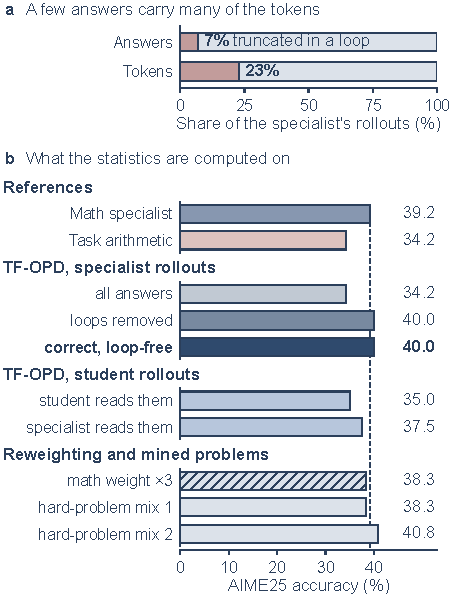
\includegraphics[width=\linewidth]{figs/rollouts.pdf}
\caption{\textbf{A few looping answers decide the hard problems.}
(a)~Answers that end in a repetition loop are a small share of the
mathematics specialist's answers and a large share of its tokens.
(b)~AIME25 accuracy of fused models by the answers their statistics use;
the dashed line is the mathematics specialist in float16, like them. The
final model of Table~\ref{tab:main} also keeps only verified code answers
(Appendix~\ref{app:ablations}).}
\label{fig:rollouts}
\end{minipage}\hfill
\begin{minipage}[t]{0.475\textwidth}
\vspace{0pt}\centering
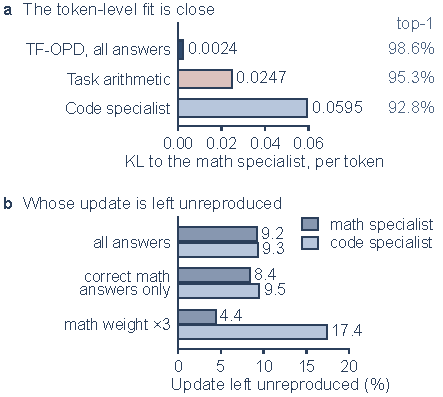
\includegraphics[width=\linewidth]{figs/diag.pdf}
\caption{\textbf{Following the specialist closely is not enough.} (a)~How
far each model is from the mathematics specialist when both read the
specialist's own correct solutions: KL divergence per token, and how often
the most likely next token agrees. (b)~Share of each specialist's update
that the fused layers fail to reproduce (Equation~\eqref{eq:diag}, median
over layers), for three choices of statistics.}
\label{fig:diag}
\end{minipage}
\end{figure}

\paragraph{A few answers never end.} Most of a specialist's answers are
ordinary reasoning that ends with a result. A few never end: the model starts
repeating itself and continues to the length limit. For the mathematics
specialist these are a small share of the answers but, being the longest, a
several times larger share of the tokens (Figure~\ref{fig:rollouts}a). Every
token counts equally in the statistics, so a fused model built from all
answers is asked, to a large extent, to behave as the specialist does inside
a loop.

\paragraph{The damage does not show token by token.} When both read the
specialist's own correct solutions, the fused model built from all answers
predicts almost the same next token as the specialist, far more closely than
task arithmetic does (Figure~\ref{fig:diag}a). Yet it scores the same as
task arithmetic on AIME25. A long derivation is decided at a few of its
steps, and an average over tokens does not see them.

\paragraph{Mathematics pays, code does not.} The repeated text concentrates
the mathematics statistics on a few directions, so each layer moves toward
the coding specialist wherever the two share inputs
(Proposition~\ref{prop:conflict}). The loss is confined to hard mathematics:
with all answers, the fused model still matches the coding specialist on both
code benchmarks and is slightly ahead of the mathematics specialist on
MATH-500 (Table~\ref{tab:abl-all}).

\subsection{Ablation study}
\label{sec:exp-selection}\label{sec:ablations}

\begin{table}[t]
\centering\small
\setlength{\tabcolsep}{8pt}
\begin{tabular}{@{}lccc@{}}
\toprule
Model & MATH-500 & HumanEval+ & MBPP+ \\
\midrule
\multicolumn{4}{@{}l}{\emph{No statistics}} \\
Task arithmetic & 92.0 & 81.7 & 69.3 \\
Low-rank sum & 91.6 & 82.9 & 68.8 \\
\midrule
\multicolumn{4}{@{}l}{\emph{\method, specialist rollouts}} \\
128 problems, 16k tokens & 92.0 & 84.8 & 68.5 \\
256 problems, 32k tokens & 93.2 & 87.2 & 70.1 \\
+ correct math answers only & 91.8 & 81.7 & 68.3 \\
+ verified code answers (final) & 90.8 & 84.1 & 67.5 \\
\midrule
\multicolumn{4}{@{}l}{\emph{\method, student rollouts}} \\
student reads its answers & 92.0 & 84.1 & 70.1 \\
+ correct math answers only & 92.4 & 84.8 & 69.0 \\
\bottomrule
\end{tabular}
\caption{\textbf{On the easier benchmarks every rule looks alike.} Accuracy
(\%), one sampled answer per problem. A row marked + adds one change to the
row above it.}
\label{tab:panel}
\end{table}

\paragraph{Which answers.} Figure~\ref{fig:rollouts}b varies only the answers
that enter the statistics. With every answer of the specialists, the fused
model is no better than task arithmetic on AIME25, and both fall short of the
mathematics specialist scored in the same format. Removing the looping
answers alone brings it level with the specialist and recovers every hard
problem that the model built from all answers loses. Keeping only correct
answers, which discards many more, changes nothing further: a finished but
wrong answer is still an example of the specialist reasoning normally.
Checking the code answers by running their tests, as the final model does,
changes code accuracy by no measurable amount (Table~\ref{tab:panel}).

\paragraph{Whose text.} On-policy distillation in the strict sense uses text
written by the student. We let a fused student answer the same problems and
compute the statistics either from the student reading its own answers or
from the mathematics specialist reading them, the closed-form analogue of
the trained objective. Neither improves on the specialist's own answers with
the looping ones removed (Figure~\ref{fig:rollouts}b).

\paragraph{Reweighting and mined problems.} Weighting mathematics three to
one in Equation~\eqref{eq:obj} recovers most of the loss, but at the coding
specialist's expense: the share of its update that the fused layers fail to
reproduce nearly doubles (Figure~\ref{fig:diag}b). Statistics from mined hard
problems give no clear gain. Selection removes the cause; the other remedies
compensate for it.

\paragraph{The merge rule.} On MATH-500 and the two code benchmarks, task
arithmetic, a low-rank variant of it and the closed form all keep both
specialists' gains and cannot be told apart (Table~\ref{tab:panel}). The
rules separate only on hard problems (Figure~\ref{fig:rollouts}b).

\paragraph{Number format.}\label{sec:exp-precision} Reinforcement learning
moves each weight by about one step of the 16-bit format the models are
released in. The closed-form update is not made of whole steps, and rounding
to that format measurably distorts it (Appendix~\ref{app:eval}), so fused
models are stored in 32-bit floats and evaluated in float16. The format
matters at the scale of our comparisons: the mathematics specialist scores
several points higher on AIME25 in its released format than in float16
(Table~\ref{tab:abl-aime}).

\subsection{Discussion}
\label{sec:discussion}

On-policy distillation is run after reinforcement learning to put several
specialists into one model. For specialists that share a base model, our
results suggest that the training in that step may not be needed. What the
trained student is asked to do, match each teacher on the text the models
generate, has an exact layer-wise solution, and that solution already gives a
model close to each teacher and more accurate on average than either. Adding
a specialist then costs its rollouts and one more term in each layer's sums;
nothing is retrained. Training remains the tool when the teachers differ in
architecture or size from the student.
